\chapter{Einleitung} % 3 Seiten

Nachfolgend wird eine kurze Einführung in das Thema gegeben und die weitere Vorgehensweise erläutert.

\section{Gegenstand der Arbeit}

Diese Arbeit verwendet die Begriffe \emph{klassische} und \emph{sicherheitskritische} Bereiche zur Differenzierung zwischen Wirtschafts- und Unternehmensteilen die keinen erhöhten Sicherheitsbedarf haben und denen die explizit höhere Anforderungen bezüglich der Sicherheit haben (z. B. Kernkraftwerke, Luft- und Raumfahrtindustrie).
Die Verletzung dieser Ansprüche kann den Verlust streng vertraulicher Daten, Gefahr für Leib und Leben oder negative Auswirkungen für die Umwelt zur Folge haben.
Die Begriffe \emph{vertikale} und \emph{horizontale Evolution} (vgl. \autoref{fig:evolution}) werden im Kontext dieser Arbeit wie folgt definiert:
\emph{Vertikale Evolution} betrifft die Anwendung agiler Entwicklungsmethoden auf die Vereinigung von Entwicklung und Betrieb von Software (DevOps).
Dahingegen beschreibt \emph{horizontale Evolution} die Implementierung von agilen Vorgehensmodellen und Methoden in sicherheitskritischen Bereichen.

\begin{figure}
  \centering
  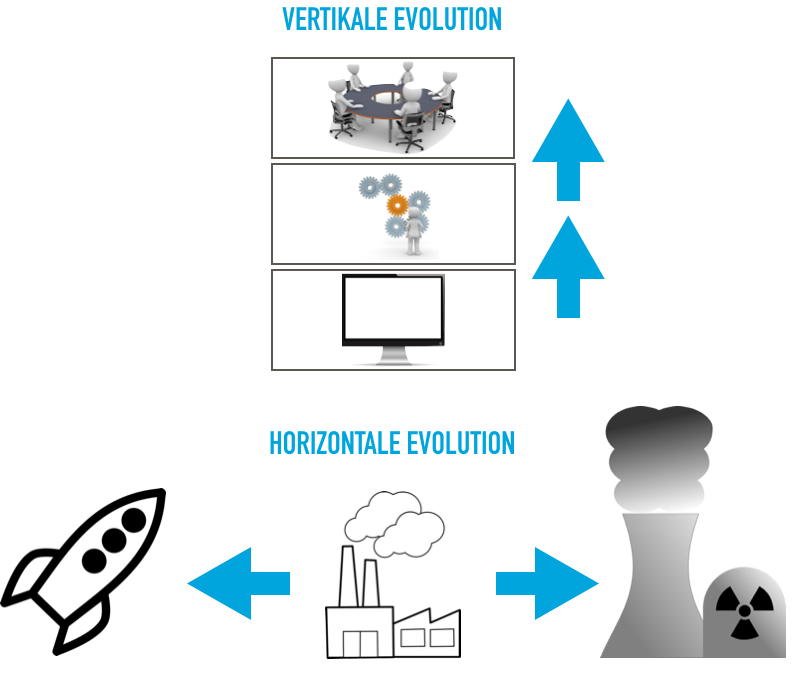
\includegraphics[width=\textwidth]{img/evolution.png}
  \caption{Vertikale und horizontale Evolution}
  \label{fig:evolution}
\end{figure}

Die agile Entwicklung ist nach diversen Studien und Umfragen bei den meisten Unternehmen im Alltag angekommen \parencite[vgl.][]{VersionOne:2015aa, HP:2015aa}. 
Damit hat sich der Trend fortgesetzt, von klassischen zu agilen Vorgehensmodellen über zu gehen \parencite[vgl.][]{Rodriguez:2012:SAL:2372251.2372275}.

Des Weiteren sind agile Vorgehensmodelle nicht nur auf die Entwicklung von Software beschränkt, sondern könnten auch auf den Betrieb von Software (DevOps) ausgeweitet werden.
Eine Fragestellung ist hierbei, welche Verbesserungen unter welchen Voraussetzungen durch die Anwendung von DevOps erreicht werden können und ob diese auch in sicherheitskritsichen Bereichen möglich sind.

In der gängigen Literatur wird meist nur auf die Anwendung von agilen Vorgehensmodellen in klassischen Bereichen eingegangen.
Insbesondere die sicherheitskritischen Bereiche, wie die Luft- und Raumfahrtindustrie, nutzen jedoch noch klassische Vorgehensmodelle.
Hier stellt sich die Frage, wie und ob diese Bereiche auch von den agilen Vorgehensmodellen profitieren können.

Die Relevanz der Fragestellung ergibt sich aus der Tatsache, dass gerade diese Bereiche oft unter hohen Lieferverzögerungen und Kostenüberschreitungen leiden.
Außerdem befindet sich beispielsweise die Raumfahrtindustrie in einem Wandel, da immer mehr private Unternehmen auf diesen Markt drängen, was einen erhöhten Wettbewerbsdruck verursacht.
Zwar finden sich zu den Themen agile Vorgehensmodelle und DevOps eine Vielzahl von Veröffentlichungen, jedoch nur sehr wenige beschäftigen sich mit der Anwendung und den Schwierigkeiten in sicherheitskritischen Bereichen.

\section{Zielsetzung}

Die vorliegende Arbeit soll untersuchen, wie und unter welchen Voraussetzungen sich DevOps einführen lässt, welche Vorteile sich dadurch für Entwicklung und Organisation ergeben und ob DevOps auch in sicherheitskritischen Bereichen Anwendung finden kann.
Außerdem soll geklärt werden, wie sich die Anwendung von agilen Vorgehensmodellen und deren Methoden auf sicherheitskritische Bereiche erweitern lässt.
Insbesondere soll untersucht werden, worin sich die klassischen und sicherheitskritischen Bereiche unterscheiden und welche Voraussetzungen geschaffen werden müssen, damit agile Methoden und DevOps eingeführt werden können.
Durch Betrachtung von Fallstudien, die die Einführung von DevOps und agilen Vorgehensmodellen in sicherheitskritischen Bereichen untersuchen, soll erarbeitet werden, welche Anpassungen an den Konzepten notwendig sind, um in diesen Bereichen sinnvoll eingesetzt werden zu können.
Abschließend sollen Schlussfolgerungen und Handlungsempfehlungen für sicherheitskritische Bereiche formuliert werden.


\section{Methodik}

Da die Arbeit bisherige Kenntnisse bezüglich sicherheitskritischen Bereichen, agilen Vorgehensmodellen und DevOps zusammentragen soll, bietet sich die Methode des \emph{Literatur-Reviews} an \parencite[vgl.][]{Fettke:2006aa}.
Die Arbeit entspricht einem natürlichsprachlichem Review mit dem Literaturfokus auf einer Kombination von Erfahrung (Anwendung in der Praxis) und der Theorie sowie empirischen Forschungsergebnissen.
Als Hauptziel sollen zentrale Aspekte der Arbeiten herausgearbeitet und Handlungsempfehlungen für die Praxis abgeleitet werden.
Hierbei beziehen die Autoren eine neutrale Haltung, wobei im Fazit eine Bewertung der Literaturergebnisse erfolgen soll.

Zur Suche wird auf die Quellen HTWG Bibliothek \parencite[][]{HTWGaa} zur Primärliteratursuche, Google Scholar und Google zur Sekundärliteratursuche zurückgegriffen.
Es werden die Stichwörter
\begin{itemize}
\item Agile
\item Agile Entwicklung / Agile Development
\item Vorgehensmodelle / Software Development Process
\item Sicherheitskritische Software / Security Critical Software
\item Luftfahrtindustrie / Air Industry
\item Raumfahrtindustrie / Space Industry
\item Softwaresicherheit / Software Security
\item Software Time To Market
\item Softwaresicherheit Anforderungen / Software Security Requirements
\item Softwarenormen / Software Standards
\item DevOps
\item Einführung DevOps / DevOps Adoption
\item DevOps Agile
\item DevOps Lean
\item DevOps Projektmanagement / DevOps Project Management
\item DevOps ITIL
\item DevOps Einsatz / DevOps Usage
\item DevOps Statistik / DevOps Statistics
\item DevOps in der Praxis / DevOps in Practice
\item DevOps Sicherheit / DevOps Security
\end{itemize}
zur Literatursuche benutzt.

Aus den Ergebnissen wird relevante Primärliteratur ausgewählt. 
Diese sollte sich mit den Kernthemen \enquote{sicherheitskritische Bereiche}, \enquote{DevOps}, \enquote{Softwarevorgehensmodelle} und \enquote{agile Vorgehensmodelle in sicherheitskritischen Bereichen} auseinandersetzen.
Bevorzugt wird Literatur ausgewählt, die in Konferenzsammlungen erschienen ist sowie die Anwendung in der Praxis untersucht.
Aus diesen Primärquellen wird mittels des Schneeballsystems (Zitate und Quellen rückwärts durchsucht) weitere relevante Literatur recherchiert.
Hier wird versucht, für den Hauptteil möglichst aktuelle Quellen zu verwenden.
Als Sekundärliteratur werden Studien und Arbeiten verwendet, die dem Rahmenwerk der Arbeit dienen und nicht die Hauptfragestellungen beantworten.
Alle Quellen werden in homogene Gruppen aufgeteilt und jeweils einige Vertreter daraus verwendet, so dass möglichst alle Aspekte der jeweiligen Thematik betrachtet werden.

Die Strukturierung der Arbeit verfolgt einen Thematisch orientierten Ansatz. 
Als Zielgruppe der Arbeit wird einerseits die Wissenschaft, als Anreiz für weitere Forschung in diesem Bereich, angesehen, als auch die Praxis, die hieraus Schlüsse über die Anwendbarkeit ziehen kann.

\section{Gang der Untersuchung}

Die Arbeit beginnt mit einer umfassenden Einführung in die Grundlagen, die klassische und agile Vorgehensmodelle vorstellt.
Des Weiteren wird der Begriff DevOps eingeführt und dessen geschichtliche Entstehung betrachtet.
Zur Verdeutlichung der Relevanz der Arbeit werden klassische und sicherheitskritische Bereiche bezüglich dem Anspruch an die Software verglichen.
Anschließend folgt die Betrachtung der vertikalen Evolution und ihrer Auswirkungen auf die Praxis.
Danach wird die horizontale Evolution analysiert, in dem zuerst die agilen Vorgehensmodelle in klassischen Bereichen und anschließend in sicherheitskritischen Bereichen untersucht werden.
Die Zusammenfassung der Arbeit und Handlungsempfehlungen für die Praxis sowie ein Ausblick auf weitere Forschungsarbeiten bilden den Schluss.



